\documentclass{article}
\usepackage[czech]{babel}
\usepackage{hyperref}
\usepackage{listings}
\usepackage{graphicx}

\title{ESP32-S3 Web Server pro ovládání LED}
\author{Autor: Jáchym Otáhal}
\date{\today}

\begin{document}

\maketitle

\section{Popis problému}
Moderní embedded systémy často vyžadují možnost vzdáleného ovládání. Cílem tohoto projektu je vytvořit webový server běžící na ESP32-S3, který umožní uživatelům měnit barvu integrované LED diody prostřednictvím webového rozhraní.

\section{Návrh řešení}
Hlavní myšlenkou je využití knihovny WebServer pro vytvoření jednoduchého webového serveru. Uživatelé mohou zadávat hodnoty RGB barev pomocí formuláře na webové stránce, které se následně aplikují na LED diodu ovládanou pomocí knihovny Adafruit NeoPixel.

\section{Popis realizace}
\subsection{Struktura kódu}
Kód obsahuje několik klíčových funkcí:
\begin{itemize}
    \item \textbf{setup()} – Inicializace Wi-Fi, LED a spuštění serveru
    \item \textbf{loop()} – Obsluha požadavků klientů
    \item \textbf{handleRoot()} – Zajištění HTML stránky pro ovládání LED
    \item \textbf{handleResponse()} - Odpověď s udanými RGB hodnotami + nastavení LED
    \item \textbf{setPixelColour()} – Nastavení barvy LED
\end{itemize}

\subsection{Použité knihovny}
Projekt využívá následující knihovny:
\begin{itemize}
    \item \textbf{WiFi.h} – Správa Wi-Fi připojení
    \item \textbf{WiFiClient.h} – Podpora Wi-Fi klienta
    \item \textbf{WebServer.h} – Implementace webového serveru
    \item \textbf{Adafruit\_NeoPixel.h} – Ovládání RGB LED diod
\end{itemize}
\\
\textbf{Kód:}
\begin{lstlisting}[language=C++]
#include <WiFi.h>
#include <WiFiClient.h>
#include <WebServer.h>
#include <Adafruit_NeoPixel.h> 

...
\end{lstlisting}

\subsection{Vlastni statementy}
\textbf{Kód:}
\begin{lstlisting}[language=C++]
...

#define inTheCaseOf if
#define otherwise else
#define duringTheTime while
#define ShallThisBooleanComeAsTrueIMustNotAllowMySelfToEndThisLoop for
#define ShoutOutLoud Serial.println

...
\end{lstlisting}

\subsection{Konfigurace HTTP serveru}
Náš webový server běží na portu 80, což je základní port pro HTTP komunikaci. Nastaví dvě adresy na kterých je responsivní.
Tyto adresy jsou / (home page) a /setpixel (pro nastavení diody). \\
\textbf{Kód:}
\begin{lstlisting}[language=C++]
...

// Set the response port
WebServer server(80);

...

// Send the homepage to the client
void handleRoot() {
  // Send the HTML form to the client
  String html = "Isn't able to fit here";
  server.send(200, "text/html", html);
}

...
\end{lstlisting}

\subsection{Nastavení LED diody}
Použitá LED dioda je připojena na pin 48 a ovládá se pomocí knihovny Adafruit NeoPixel.
Po odeslání nastavení pomocí handleResponse() se zvolá funkce setPixelsColor(), která nastavuje hodnoty led diod. \\ 
\begin{figure}[h]
  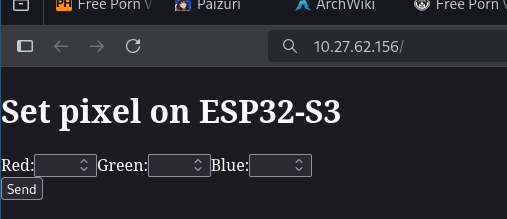
\includegraphics{Pictures/root.png}
\end{figure}
\\
\textbf{Kód:}
\begin{lstlisting}[language=C++]
...

#define PIN_LED 48
#define PIXNUM 1
Adafruit_NeoPixel pixels(PIXNUM, PIN_LED, NEO_GRB + NEO_KHZ800);

...

void setPixelsColor(int red, int green, int blue) {
  ShallThisBooleanComeAsTrueIMustNotAllowMySelfToEndThisLoop(
  int i=0; i < PIXNUM; i++) {
    pixels.setPixelColor(i, pixels.Color(red, green, blue));
    pixels.show();
  }
}

...

void handleResponse() {
  inTheCaseOf (server.method() == HTTP_POST) {
    String red = server.arg("red");
    String blue = server.arg("blue");
    String green = server.arg("green");
    shoutOutLoud("Received settings: " + red + " " + blue + " " + green);
    

    setPixelsColor(red.toInt(), green.toInt(), blue.toInt());

    // Send a response back to the client
    server.send(200, "text/html", "Here Goes HTML");
  } otherwise {
    server.send(405, "text/html", "<h1>Method Not Allowed</h1>");
  }
}

...
\end{lstlisting}

\section{Testování a vyhodnocení}
Testování bylo provedeno s ESP32-S3 a připojenou LED diodou. 
Webový server úspěšně načítal HTML stránku a umožňoval měnit barvu 
LED diody dle zadaných hodnot. Odezva systému byla rychlá a stabilní. 
Možná vylepšení zahrnují přepsání do ESP-IDF nebo implementaci 
ovládání přes MQTT.

\end{document}
